%ju 16-Dez-22 03-Hochvolt.tex
\textbf{Reichweite Batterie} $\sim 770~km$ (MERCEDES EQS (2021) -
S-KLASSE \footnote{\url{https://www.auto-motor-und-sport.de/})} (Stand:
Mai/2022)

\textbf{Spannung Bordnetz} $400~V - 800~V$ (Porsche Taycan, Audi
e-tron)

\textbf{Batterie laden (Möglichkeiten)}

\begin{figure}[!ht]% hier: !ht
\centering
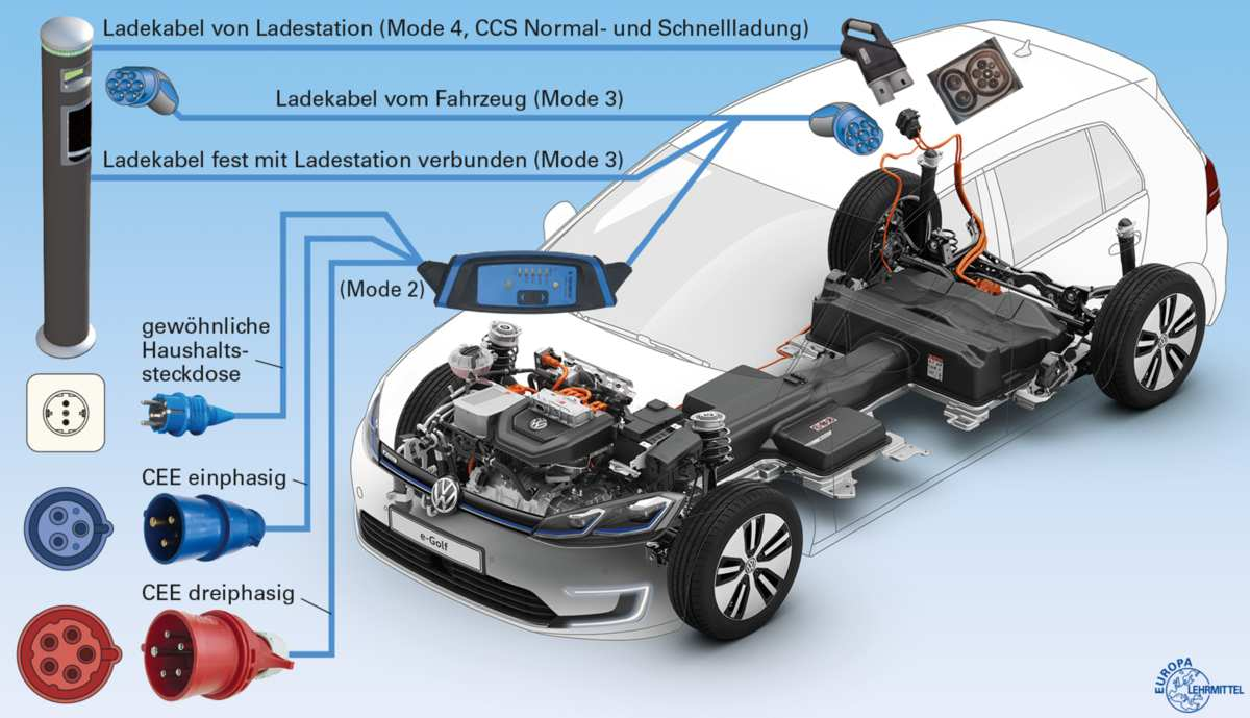
\includegraphics[width=0.7\textwidth]{images/HV/HV-1.pdf}
\caption{Ladestecker, Quelle: Europa-Verlag}
%\label{fig:}%% anpassen
\end{figure}

\begin{itemize}
\item
  AC (Wechselstrom) 230 V (1-Phase), umwandeln in Gleichstrom
  ($3,7~KW/h$)

  \begin{itemize}
  \item
    Ladestecker: Typ-2-Ladekabel mit ICCB
  \end{itemize}
\item
  AC (Wechselstrom) 380 V (3-Phasen), umwandeln in Gleichstrom
  ($11 \dots 22~KW/h$)

  \begin{itemize}
  \item
    Ladestecker: Typ-2
  \end{itemize}
\item
  DC (Gleichstrom)

  \begin{itemize}
  \item
    Ladestecker: CHAdeMO ($50~KW/h$) / CSS ($50 \dots 350~KW/h$)
  \end{itemize}
\end{itemize}

\textbf{Was ist ein Hybridfahrzeug? Hybrid-Vehicle (HV)} ist mit
mindestens zwei unterschiedlichen Energiewandlern und -speichern für den
Antrieb des Fahrzeuges ausgestattet.

Beispiel: Verbrennungsmotor und Kraftstofftank \& E-Motor und
HV-Batterie

\textbf{Was ist Hochvolt?} Ab einer Wechselspannung von AC
> 30 V und einer Gleichspannung von DC > 60 V.

\textbf{IT-Netz} IT steht für isoliert und Terra (von der Erde
isoliertes System): Das HV-System ist sowohl wechsel- als auch
gleichstromseitig von der Fahrzeugmasse galvanisch getrennt oder
isoliert (nicht geehrtes Stromnetz).

\textbf{Rekuperation (Regeneration)} Bremsenergierückgewinnung,
Bremsenergie wird in elektrische Energie umgewandelt.

\textbf{Range-Extender} Reichweiten verlängern

\textbf{Boost} Drehmomentunterstützung

\section{Was sind HV-eigensichere
Fahrzeuge?}\label{was-sind-hv-eigensichere-fahrzeuge}

Für den Benutzer durch technische Maßnahmen ein vollständiger Berühr-
und Lichtbogenschutz gegenüber dem HV-System gewährleistet ist.

\begin{itemize}
\item
  System überwacht sich selbst
\item
  Serienfahrzeug (Direkt vom Hersteller auf die Straße)
\item
  Sicherheitslinie (Pkw)
\item
  \textbf{Außer:} Lkw, Busse, Eigenbau (Vorsicht beim Umrüsten und
  Nachrüsten), Unfallfahrzeug
\end{itemize}

\section{Qualifikationsstufen}\label{qualifikationsstufen}

Jeder \textbf{Gewerbetreibende} benötigt die Stufe-S, um ein HV-Fahrzeug
bewegen zu dürfen.

\textbf{Unterweisung} einmal jährlich für Gesellen und halbjährlich für
Lehrlinge. $\to$ Person sensibilisieren auf jedes Fahrzeug einzeln.

\textbf{Wie heißt die neue Sicherheitsverordnung?}

DGUV 209-093 (Deutsche gesetzliche Unfallversicherung) Qualifizierung
für Arbeiten an Fahrzeugen mit HV-Systemen.

\subsection{Qualifikationsstufen}\label{qualifikationsstufen-1}

\begin{itemize}
\item
  \textbf{Stufe S} sensibilisierte Person (Bedienen von Fahrzeugen mit
  HV-System)
\item
  \textbf{Stufe 1S} fachkundige unterwiesene Person (Motto: Hände weg
  von Orange!)
\item
  \textbf{Stufe 2S} fachkundige Person (alle arbeiten, aber nicht unter
  Spannung, Freischalten)
\item
  \textbf{Stufe 3S} fachkundige Person -- für Arbeiten unter Spannung
  stehenden HV-System (Energiespeicher öffnen), erste Hilfe-Schein
\end{itemize}

\textbf{Welche Qualifikationen sind für folgende Arbeiten notwendig?}

\begin{enumerate}
\item
  \textbf{VW E-Golf kommt zum Räderwechsel}

  \begin{itemize}
  \item
    Fachkundige unterwiesene Person
  \end{itemize}
\item
  \textbf{Lehrling soll VW E-Golf in eine andere Filiale fahren}

  \begin{itemize}
  \item
    Sensibilisierte Person
  \end{itemize}
\item
  \textbf{Beim Smart ED soll der Klimakompressor getauscht werden}

  \begin{itemize}
  \item
    Fall 1: Wenn nicht freigeschaltet ist $\to$ Stufe 2S
  \item
    Fall 2: Wenn freigeschaltet ist $\to$ Stufe 1S + Klimaschein
  \end{itemize}
\item
  \textbf{Tesla Model S braucht eine neue HV-Batterie}

  \begin{itemize}
  \item
    Fachkundige Person
  \end{itemize}
\item
  \textbf{Nach Unfall lässt sich Mercedes Vito E-Cell nicht mehr über
  Service-Disconnect-Stecker spannungsfrei schalten}

  \begin{itemize}
  \item
    Fachkundige Person -- für Arbeiten unter Spannung stehenden
    HV-System
  \end{itemize}
\end{enumerate}

\newpage

\section{Erkläre das Freischalten des
HV-Systems?}\label{erklaere-das-freischalten-des-hv-systems}

\begin{figure}[!ht]% hier: !ht
\centering
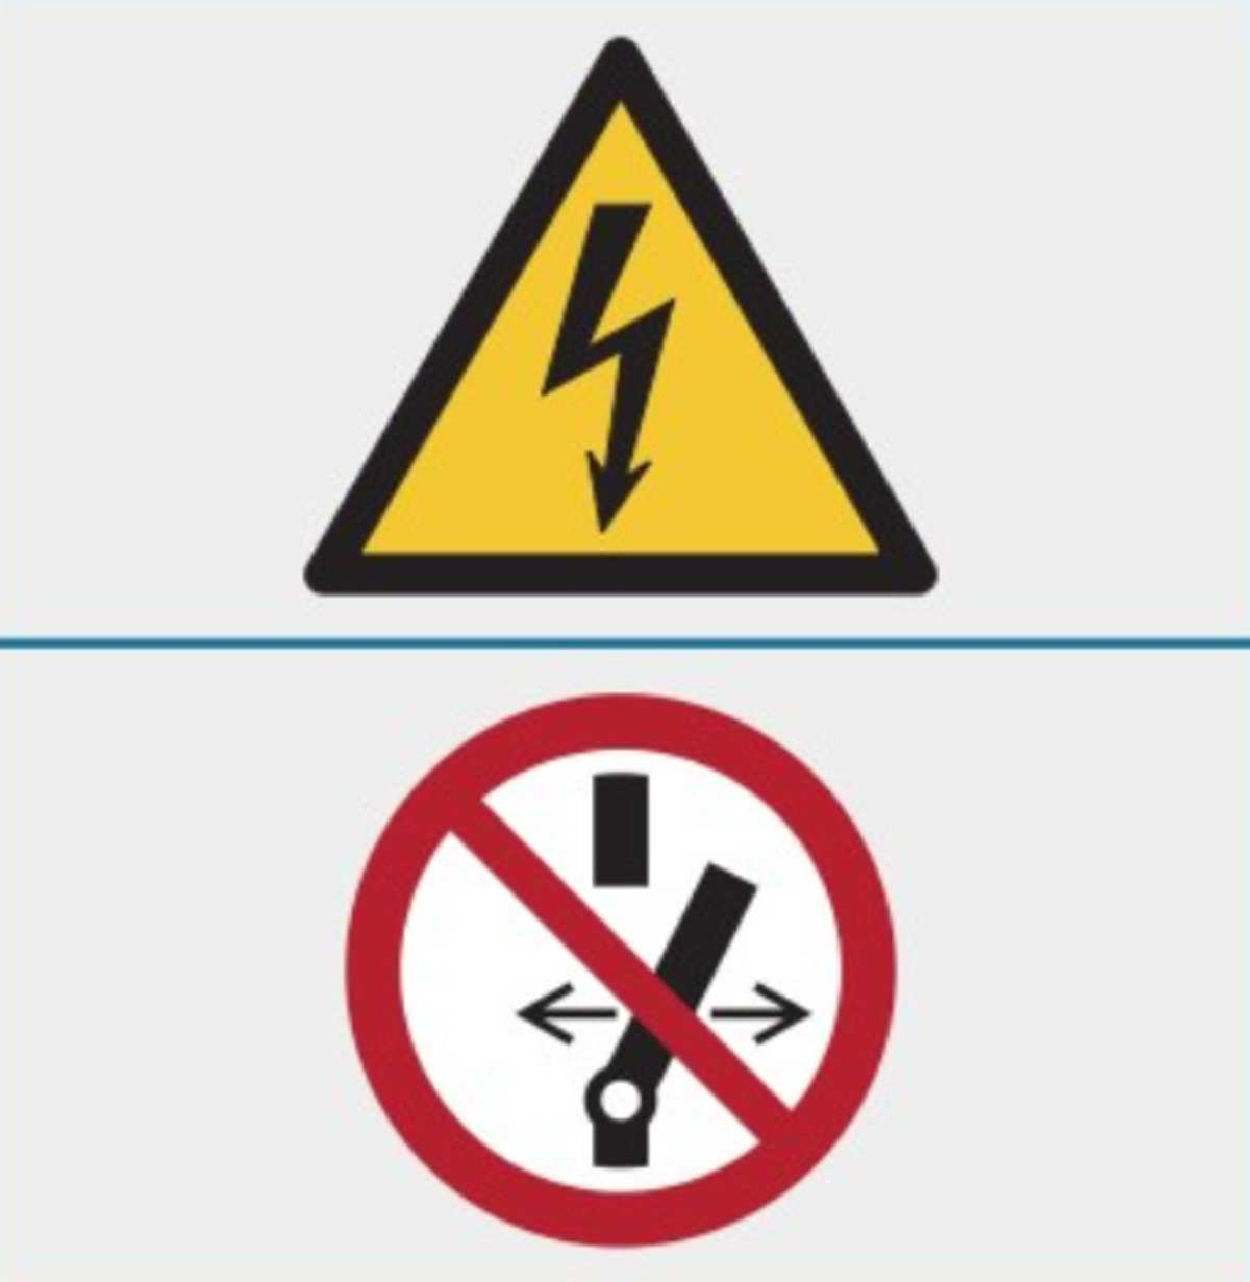
\includegraphics[width=0.2\textwidth]{images/HV/HV-8.pdf}
\caption{Blitzhütchen (Gefährliche Spannung) + Gegen Wiedereinschalten
gesichert, Quelle: Europa-Verlag}
%\label{fig:}%% anpassen
\end{figure}

Kunde kommt mit E-Auto in die Werkstatt. Was passiert jetzt?

Beginn Gefahrübergang: mit Schlüsselübergabe + Normalauftrag
(Garantieauftrag) unterschrieben.

\textbf{Probefahrt} ja der Fehler ist aktuell.

Vorgaben des Herstellers beachten!

\begin{enumerate}
\item
  Blitzhütchen >>Hochvolt<< mit Magnet aufs Dach
\item
  Fahrzeug in Werkstatt fahren

  \begin{itemize}
  \item
    fester Platz für HV-Fahrzeug
  \item
    HV-Werkzeug, Rettungshaken, Feuerlöscher, Defibrillator
    (Herzrhythmusstörung beseitigen, Stromstoß)
  \end{itemize}
\item
  Abschranken

  \begin{itemize}
  \item
    Gefahren absperren im Abstand 1,50 m um das Fahrzeug herum
  \item
    Bedeutung von gelb/schwarzes Band - langfristig oder rot/weiß Band -
    kurzfristig
  \end{itemize}
\item
  Hinweisblatt rot >>Hochvolt-Spannungen sind eingeschaltet<< auf die
  Windschutzscheibe kleben, mit Namen und Telefonnummer
\item
  Diagnosetester - Fehlerspeicher auslesen
\item
  Zündung ausschalten und Zündschlüssel entfernen (mind. 10 m
  Entfernung) und wegschließen
\item
  Sicherheitshandschuhe prüfen und anziehen, Schutzbrille, lange
  Kleidung ohne Reißverschluss (Vgl. Körperwiderstand)
\item
  Minuspol der 12 V-Batterie abklemmen (Motorhaube, Türen und Kofferraum
  vorher öffnen)
\item
  Warten 5 Minuten $\to$ bis Kondensatoren sich entladen von Bordnetz
  und HV-System

  \begin{itemize}
  \item
    Sicherheitslinie wird geöffnet
  \item
    Trennrelais öffnen und schalten Spannung ab
  \item
    Kondensatoren entladen sich
  \end{itemize}
\item
  Service-Disconnect-Stecker der HV-Batterie abziehen, falls nicht
  vorhanden, Sicherheitslinie unterbrechen
\item
  Zündschlüssel und Disconnect-Stecker wegschließen (mind. 10 m
  Entfernung) und Fahrzeug gegen Wiedereinschalten sichern
\item
  Messen mit dem Duspol (geeignetes Messgerät auswählen, Zweipoliger
  Spannungsprüfer)

  \begin{itemize}
  \item
    Messgerät an sicherer Spannungsquelle überprüfen:
    Hochspannungsbereich 230 V-Steckdose, Niederspannungsbereich 12
    V-Batterie
  \item
    Spannungsfreiheit überprüfen: am Inverter alle drei Phasen messen
  \item
    Messgerät nochmals überprüfen (gleiche Spannungsquelle)
  \item
    Spannungsfreiheit festgestellt
  \end{itemize}
\item
  Protokoll über die Freischaltung führen (Was wurde gemacht? Wie wurde
  das Fahrzeug übergeben?)
\item
  Hinweisblatt weiß >>Hochvolt-Spannungen sind sicher ausgeschaltet<<
  auf die Windschutzscheibe kleben, mit Namen und Telefonnummer
\item
  Jetzt kann gearbeitet werden.
\end{enumerate}

\textbf{HV-Interlock} Pilotlinie, Sicherheitslinie (überwacht die
HV-Steckverbindungen)

\begin{figure}[!ht]% hier: !ht
\centering
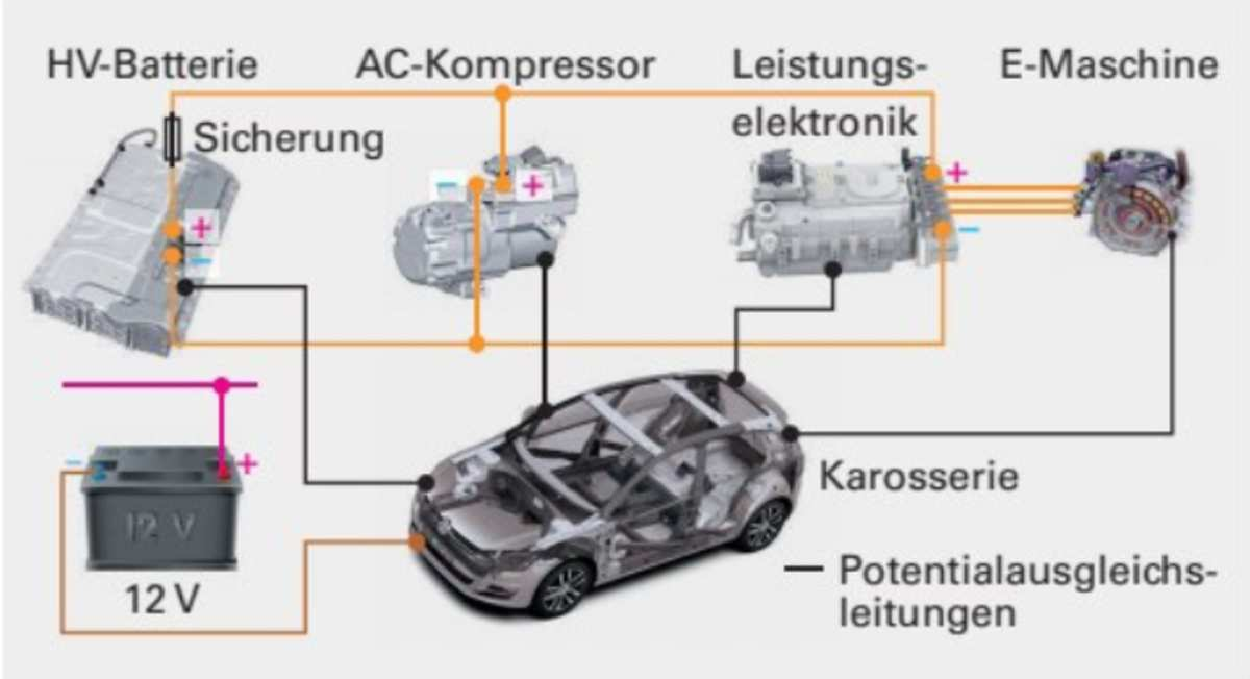
\includegraphics[width=0.4\textwidth]{images/HV/HV-7.pdf}
\caption{Sicherheitslinie, Quelle: Europa-Verlag}
%\label{fig:}%% anpassen
\end{figure}

\subsection{Wie hoch ist der Körperwiderstand ab einer Spannung von 100
V?}\label{wie-hoch-ist-der-koerperwiderstand-ab-einer-spannung-von-100-v}

Berührung der beiden Batteriepole

\begin{itemize}
\item
  $1000~\Omega$ von Hand-zu-Hand oder Hand-zu-Fuß
\item
  $450~\Omega$ von Hand-zu-Brust
\item
  $\text{Körperstrom} = \frac{400~V}{1000~\Omega} = 400~mA$ der
  absolut tödlich wäre.
\end{itemize}

Ein Strom von beispielsweise $50~mA$ kann zur Muskelverkrampfung
führen, sodass sich die Person nicht mehr selbstständig von der
Spannungsquelle lösen kann. Schon nach wenigen Sekunden könnte es auch
bei niedrigen Strömen zu tödlichen Unfällen kommen. (Einwirkzeit)

\textbf{Wovon hängt es ab, welche Schäden der elektrische Strom im
menschlichen Körper verursacht?}

\begin{itemize}
\item
  der Stromstärke und
\item
  der Zeit, für die der Strom den Körper durchfließt
\end{itemize}

\subsection{Sicherheitshandschuhe
prüfen}\label{sicherheitshandschuhe-pruefen}

\begin{itemize}
\item
  vor jedem Freischalten
\item
  Handschuh aufdrehen und auf Dichtheit prüfen oder Prüfgerät
\item
  keine Verfärbung oder Punkte
\item
  Aufdruck vollständig
\end{itemize}

Sicherheitsklasse 0 sind bis 1000 V zugelassen.

\section{Elektromotoren -
Drehstrommotor}\label{elektromotoren-drehstrommotor}

Sind bürstenlose Motoren (d.~h. keine Kohlestifte = Kohlebürsten; kein
Schleifring).

\textbf{Drehstrommotor} wird mit Dreiphasenwechselspannung betrieben,
der in drei Leitern eine periodisch um 120° versetzte Spannung anlegt.
Dadurch werden in den Statorspulen Magnetfelder induziert, die eine
Bewegung im Rotor erzeugen. Ein umlaufendes Magnetfeld nimmt einen
magnetischen Rotor mit, sodass es zu einer Drehbewegung kommt.

\begin{itemize}
\item
  \textbf{Stator} steht
\item
  \textbf{Rotor} dreht sich
\end{itemize}

\newpage

\textbf{Was ist ein Drehfeld?}

\begin{figure}[!ht]% hier: !ht
\centering
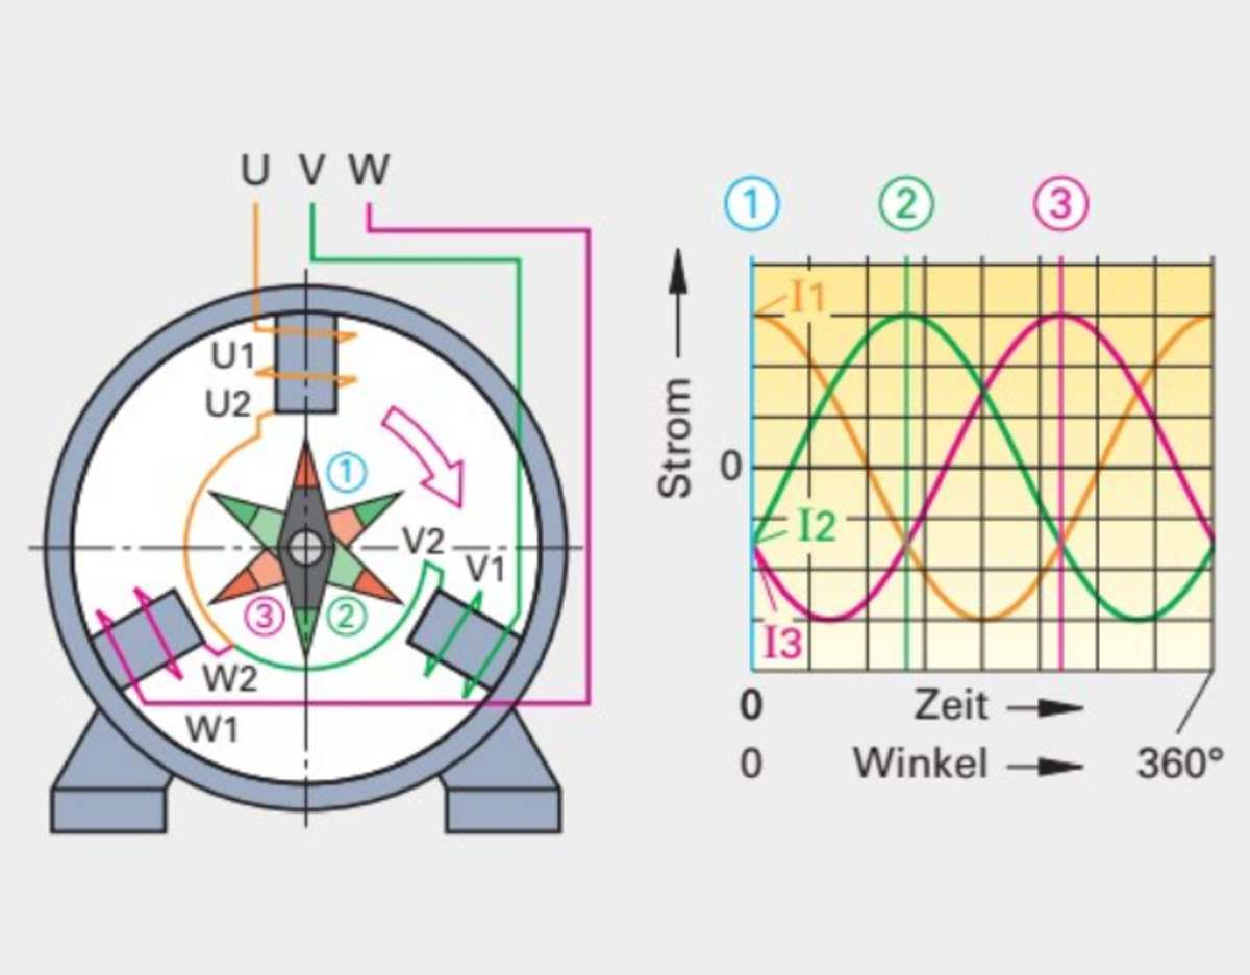
\includegraphics[width=0.3\textwidth]{images/HV/HV-9.pdf}
\caption{Drehfeld, Quelle: Europa-Verlag}
%\label{fig:}%% anpassen
\end{figure}

Ein Magnetfeld das um den Rotor wandert (rotierendes Magnetfeld).

\subsection{Synchronmotor (Prüfung)}\label{synchronmotor-pruefung}

\begin{figure}[!ht]% hier: !ht
\centering
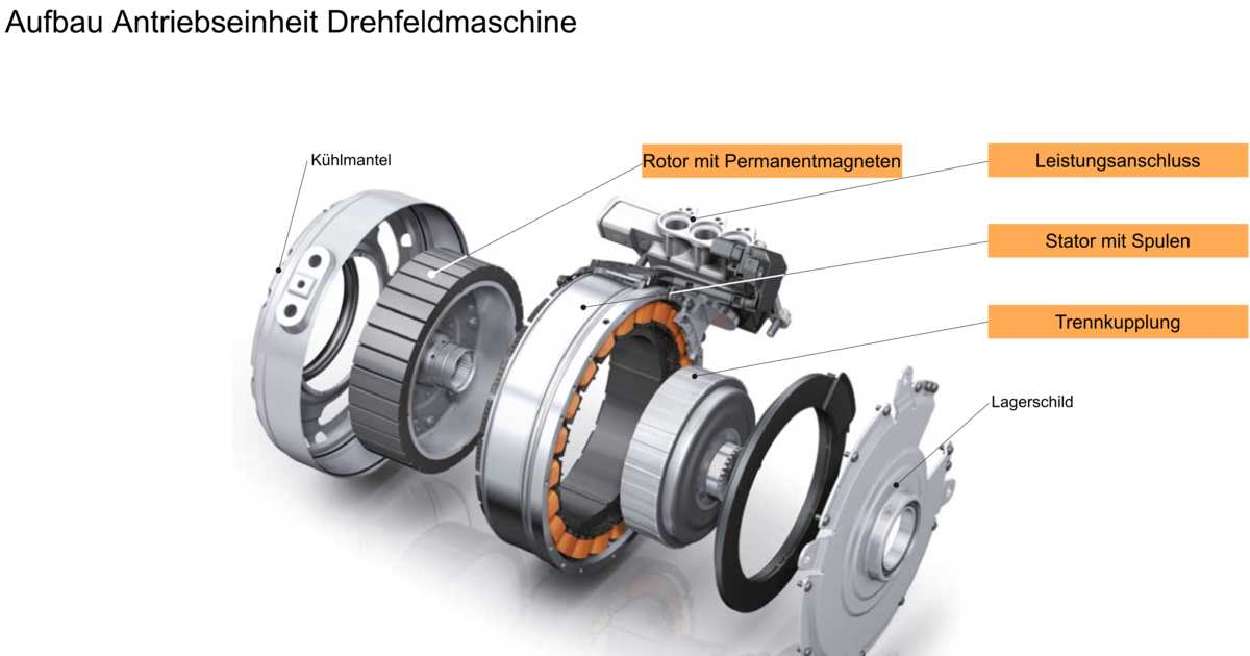
\includegraphics[width=0.6\textwidth]{images/HV/HV-6.pdf}
\caption{Synchronmotor, Quelle: Europa-Verlag}
%\label{fig:}%% anpassen
\end{figure}

Der Frequenzumrichter legt eine Dreiphasenwechselspannung an die
Erregerspulen. Das dadurch erzeugte magnetische Drehfeld des Stators
setzt den Rotor in Bewegung.

PSM (Permanenterregt)

\begin{itemize}
\item
  \textbf{Stator} die elektromagnetischen Spulen (Erregerspulen) werden
  bestromt und es entsteht ein magnetisches Drehfeld (Erregerfeld)
\item
  \textbf{Rotor} Magnetfeld wird erzeugt durch Dauermagnet, der vom
  Drehfeld direkt mitgenommen wird.
\item
  Stator = Rotor (Drehzahl, mit gleicher Geschwindigkeit)
\item
  Ansteuerung: über Inverter / IGBTs
\end{itemize}

FSM (Fremderregt)

\begin{itemize}
\item
  \textbf{Stator} elektromagnetische Spule
\item
  \textbf{Rotor} Magnetfeld wird erzeugt durch Fremderregung,
  elektromagnetische Spule
\end{itemize}

\subsection{Asynchronmotor (Prüfung)}\label{asynchronmotor-pruefung}

\begin{figure}[!ht]% hier: !ht
\centering
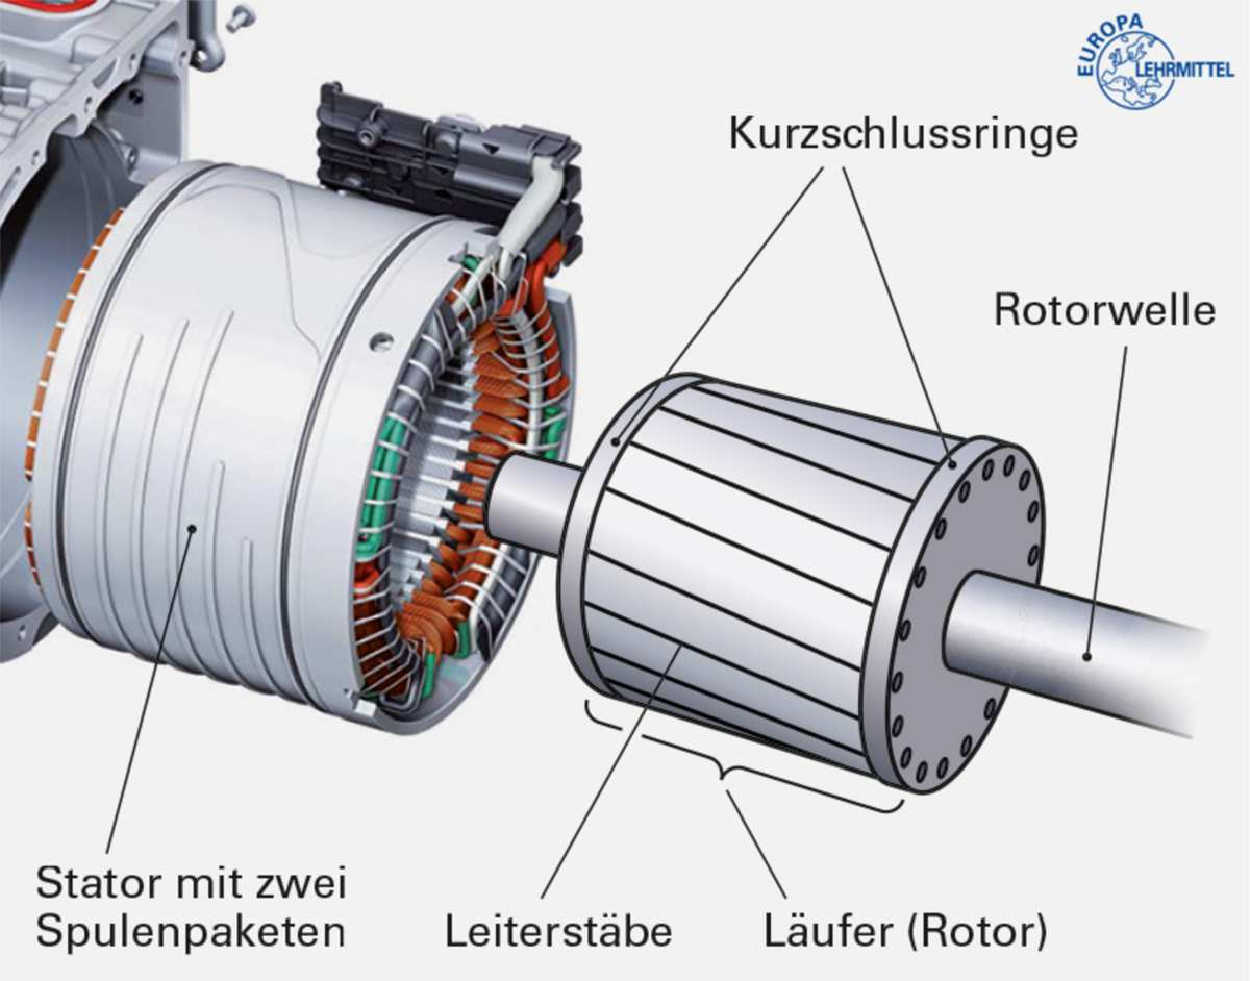
\includegraphics[width=0.4\textwidth]{images/HV/HV-5.pdf}
\caption{Asynchronmotor, Quelle: Europa-Verlag}
%\label{fig:}%% anpassen
\end{figure}

Das Magnetfeld des Rotors muss erst erzeugt werden.

ASM (Induktionsmotor)

\begin{itemize}
\item
  \textbf{Stator} die elektromagnetischen Spulen (Erregerspulen) werden
  bestromt und es entsteht ein magnetisches Drehfeld (Erregerfeld)
\item
  \textbf{Rotor} Kurzschlussläufer (Bauform, Käfigläufer), die Enden der
  Spulen werden gemeinsam verbunden. Die induzierte Spannung wird
  kurzgeschlossen und es fließt ein hoher Strom, der das Magnetfeld
  erzeugt. Rotor wird vom Drehfeld mitgenommen (mit Schlupf)
\item
  Stator $\neq$ Rotor (Drehzahl, nicht mit gleicher Geschwindigkeit)
\item
  Stator = Rotor (Kraft NULL)
\end{itemize}

Die Drehzahl wird über die Frequenz des Erregerfeldes eingestellt.

\textbf{Schlupf} unterschied zwischen Rotordrehzahl und Drehzahl des
Erregerfeldes. Asynchronmotoren laufen immer etwas langsamer als das
angelegte Erregerfeld.

\newpage

\section{HV-Komponenten}\label{hv-komponenten}

\begin{figure}[!ht]% hier: !ht
\centering
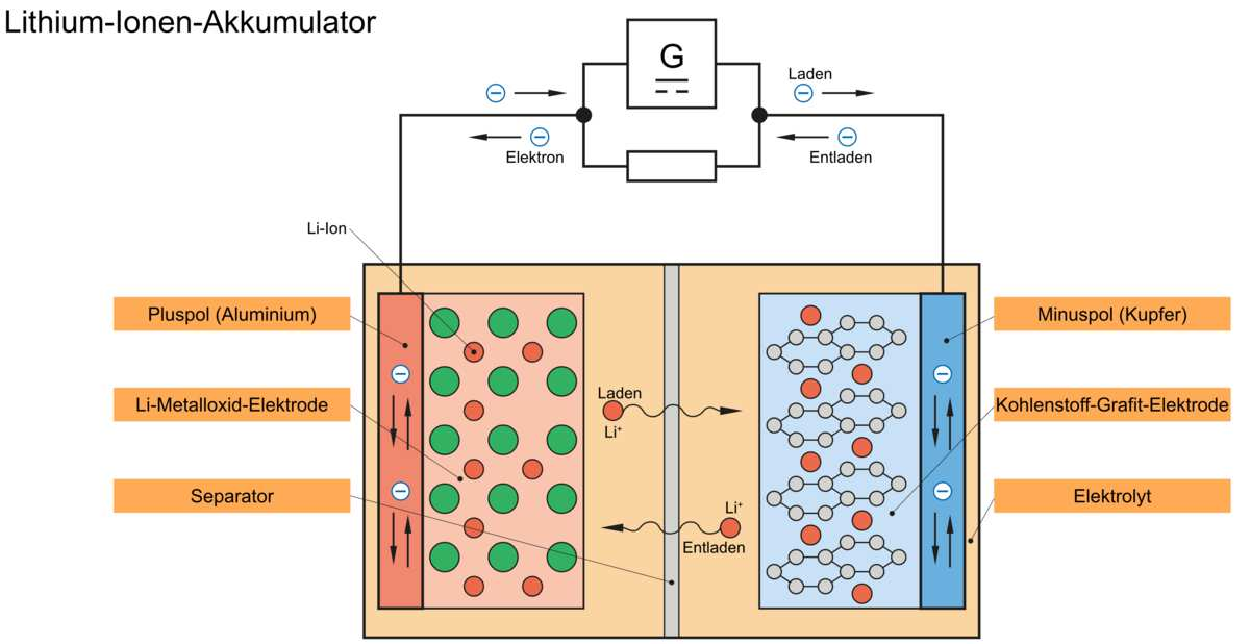
\includegraphics[width=0.5\textwidth]{images/HV/HV-3.pdf}
\caption{Lithium-Ionen-Batterie, Quelle: Europa-Verlag}
%\label{fig:}%% anpassen
\end{figure}

\begin{enumerate}
\item
  \textbf{HV-Batterie} Lithium-Ionen, Nickel-Metallhydrid
\item
  \textbf{DC/DC-Wandler} (Konverter, Gleichstromwandler)
  Spannungswandler zwischen HV-Netz und 12-V-Bordnetz
\item
  \textbf{Inverter} (Pulswechselrichter)

  \begin{itemize}
  \item
    Leistungselektronik

    \begin{itemize}
    \item
      Umwandlung DC $\to$ AC, Gleichrichten AC $\to$ DC
    \item
      Laden der HV-Batterie
    \item
      Antrieb der Motorgeneratoren (MG, E-Maschine) und Klimakompressor
    \item
      \textbf{IGBT} (Aufbau: Mosfet + Bipolarer Transistor), Wie?
      $\to$ Mit PWM-Signal werden die Spulen der Elektromotoren
      angesteuert. Durch eine Frequenzweitenmodulation lässt sich die
      Frequenz des Wechselstroms verändern.
    \end{itemize}
  \end{itemize}
\item
  \textbf{Ladeelektronik} Batterie-Balancing

  \begin{itemize}
  \item
    Aktiv Balancing (Ladungsausgleich der einzelnen Batteriezellen)
  \item
    Passiv Balancing, wenn Zelle bei 100 \%, dann über Widerstand
    (Wärme)
  \end{itemize}
\item
  \textbf{Batteriemanagementsystem} (BMS) Batterieüberwachung
\item
  \textbf{E-Maschine} (E-Motor / Generator)
\end{enumerate}

\textbf{SOC} Ladezustand vom Akku

\textbf{SOH} Alterungszustand vom Akku

\textbf{Energiefluss}

\begin{enumerate}
\item
  \textbf{Elektroantrieb} HV-Batterie - Inverter - E-Motor
\item
  \textbf{Generatorbetrieb} Generator - Gleichrichter - HV-Batterie
\item
  \textbf{Bordnetzversorgung} MG - DC/DC Wandler - 12-V-Batterie
\item
  \textbf{AC-Laden} Ladesteckdose - Gleichrichter - HV-Batterie
\end{enumerate}

\newpage

\section{Hauptrelais oder Trennrelais oder
Sicherheitsrelais}\label{hauptrelais-oder-trennrelais-oder-sicherheitsrelais}

\begin{figure}[!ht]% hier: !ht
\centering
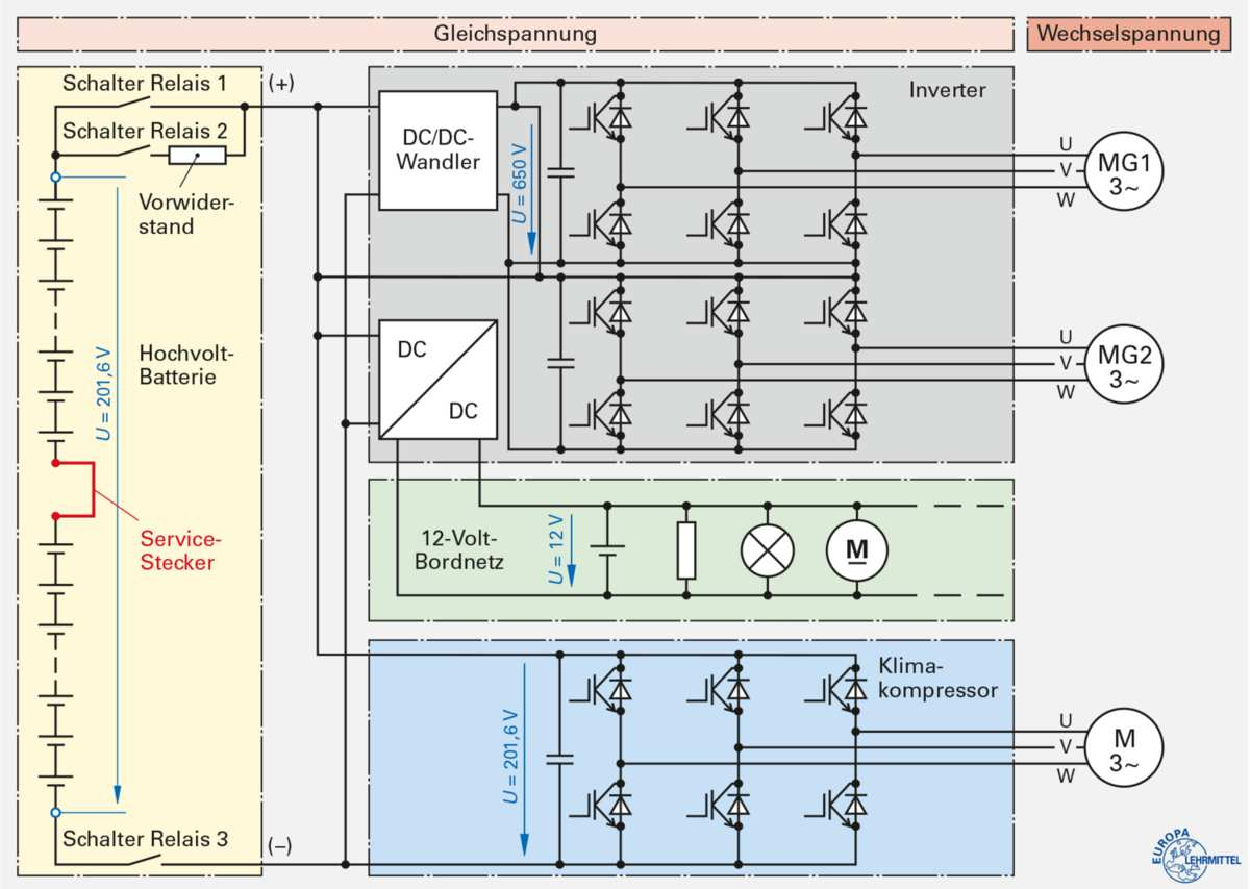
\includegraphics[width=0.7\textwidth]{images/HV/HV-2.pdf}
\caption{Hauptrelais, Quelle: Europa-Verlag}
%\label{fig:}%% anpassen
\end{figure}

\textbf{Einschalten der Zündung und betriebsbereiten Zustand}

\begin{itemize}
\item
  Relais 3 ($\text{HV}_-$) und Relais 1 ($\text{HV}_+$) mit
  Widerstand (begrenzter Stromfluss für Kondensatoren) geschlossen und
  Relais 2 offen
\item
  Lädt die Kondensatoren auf
\item
  Isolationsprüfung (Isolationsfehler oder Stecker ab $\to$
  Sicherheitslinie offen)
\item
  Fahrbereit
\end{itemize}

\textbf{Ausschalten der Zündung} trennen die Relais die HV-Spannung vom
HV-Netz

\begin{figure}[!ht]% hier: !ht
\centering
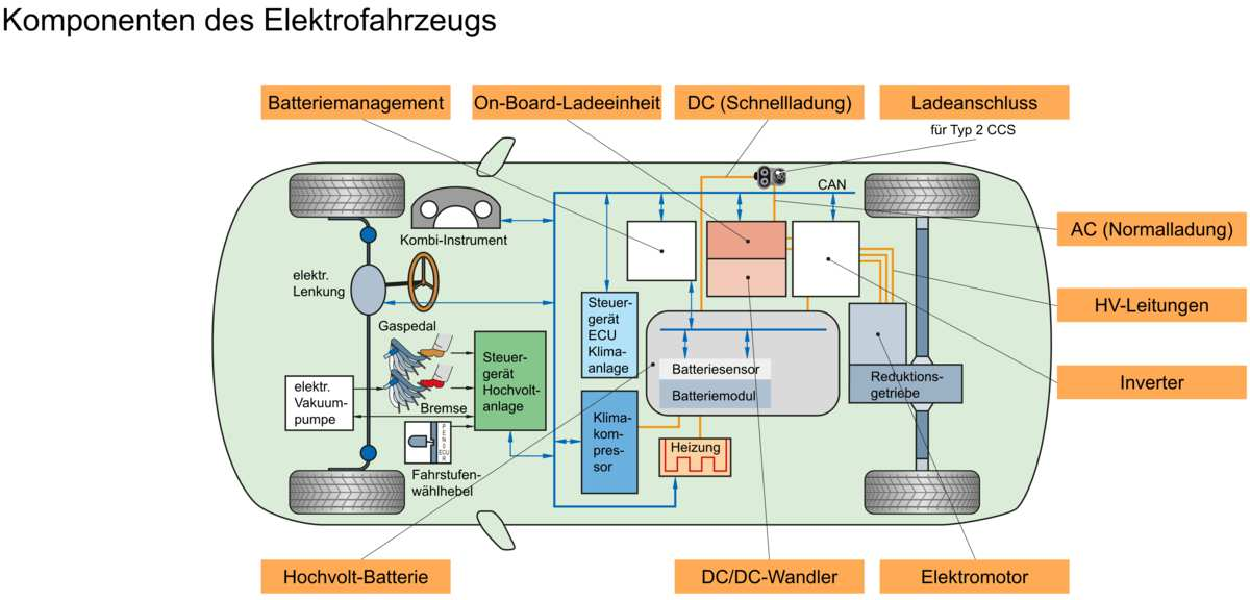
\includegraphics[width=0.7\textwidth]{images/HV/HV-4.pdf}
\caption{Elektrofahrzeug, Quelle: Europa-Verlag}
%\label{fig:}%% anpassen
\end{figure}
